%! TeX program = lualatex
%----------------------------------------------------------------------------------------
%    PACKAGES AND THEMES
%----------------------------------------------------------------------------------------

\documentclass[aspectratio=169,xcolor=dvipsnames,10pt]{beamer}
\usetheme{SimplePlus}

\usepackage{hyperref}
\usepackage{graphicx} % Allows including images
\usepackage{booktabs} % Allows the use of \toprule, \midrule and \bottomrule in tables
\usepackage{bbm}
\usepackage{bm}
\usepackage{mathtools}
\usepackage{amsthm}
\usepackage{tikz-cd}
\usepackage{listings}

%%%%%%% JULIA %%%%%%%%%%
\usepackage{fontspec}

\newfontfamily\JuliaMono{JuliaMono}[
	UprightFont = *-Regular,
	BoldFont = *-Bold,
	Path =/Users/davibarreira/Library/Fonts/,
	Extension = .ttf]
\newfontface\JuliaMonoRegular{JuliaMono-Regular}
\newfontface\JuliaMonoBold{JuliaMono-Bold}
% \setmonofont{JuliaMono-Light}[Contextuals=Alternate]


\input{julia_listings}
\input{julia_listings_unicode}

\lstdefinelanguage{JuliaLocal}{
    language = Julia, % inherit Julia lang. to add keywords
}
% \newcommand{\pc}[1]{\lstinline[style=julia]{#1}}
\newcommand{\pc}[1]{\lstinline[style=juliasmall]{#1}}
\newcommand{\pcsmall}[1]{\lstinline[style=juliasmall]{#1}}
\renewcommand{\lstlistingname}{Code}
%%%%%%%%%%%%%%%%%%%%%%%%


\theoremstyle{definition}
\newtheorem{proposition}{Proposition}

\usepackage[square,numbers]{natbib}
\newcommand*{\QEDA}{\hfill\ensuremath{\blacksquare}}%
\newcommand*{\QEDB}{\hfill\ensuremath{\square}}%

%----------------------------------------------------------------------------------------
%    TITLE PAGE
%----------------------------------------------------------------------------------------

\title{Data Visualization From a Category Theory Perspective}
\subtitle{}

\author{Davi Sales Barreira, Asla Medeiros e Sá}

\institute
{
    FGV - EMAp, IMPATech
}
\date{\today} % Date, can be changed to a custom date

%----------------------------------------------------------------------------------------
%    PRESENTATION SLIDES
%----------------------------------------------------------------------------------------
\setbeamertemplate{blocks}[default]
\setbeamercolor{block title}{fg=white, bg=RoyalBlue}
\setbeamercolor{block body}{fg=black, bg=white}

\begin{document}

\begin{frame}
    % Print the title page as the first slide
    \titlepage
\end{frame}

%------------------------------------------------
\begin{frame}{Table of contents}
    \begin{enumerate}
        \item Category Theory behind Vizagrams
        \item Vizagrams Hands-on
    \end{enumerate}
\end{frame}

\begin{frame}{Introduction}
    \centering
    Balance expressiveness and abstraction in data visualization frameworks.
    \\[1em]
    
\includegraphics[width=0.8\textwidth]{./figures/expressiveness.pdf}
\end{frame}

\begin{frame}{Introduction}
    \centering
    Visualization grammars often come short in terms of expressiveness, e.g., composite visualizations and visualizations with custom marks.
    \\[1em]
    \includegraphics[width=\textwidth]{figs/compvis.png}
\end{frame}

\begin{frame}{Introduction}
    \centering
    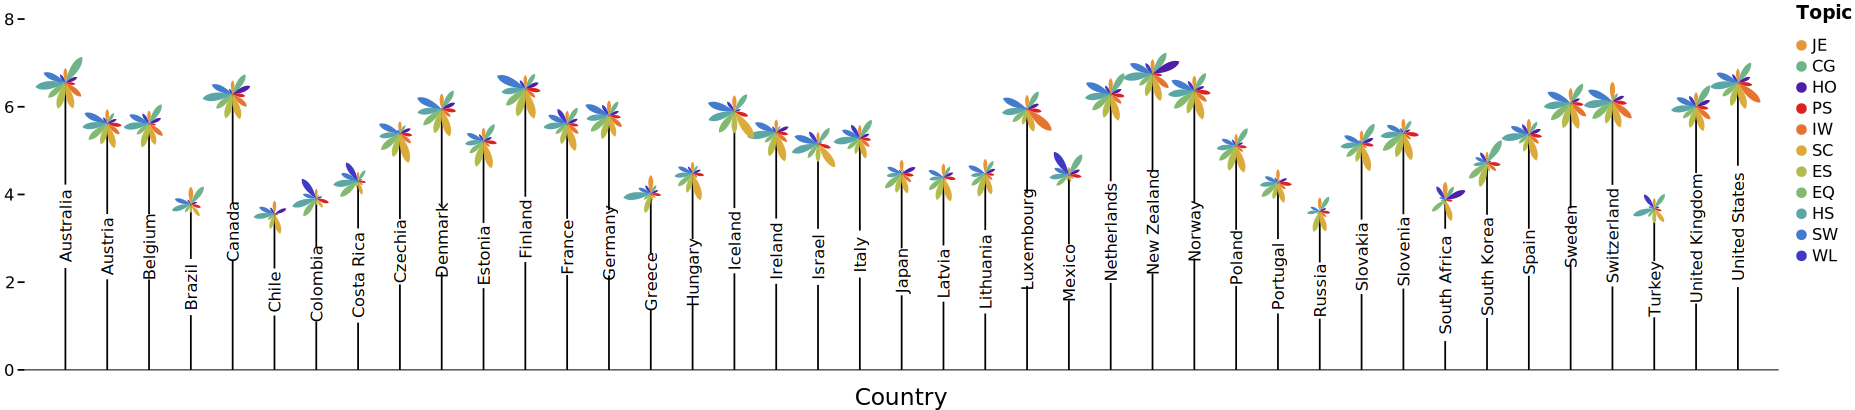
\includegraphics[width=\textwidth]{./figs/moritz.pdf}
\end{frame}

\begin{frame}{Introduction}
    \centering
    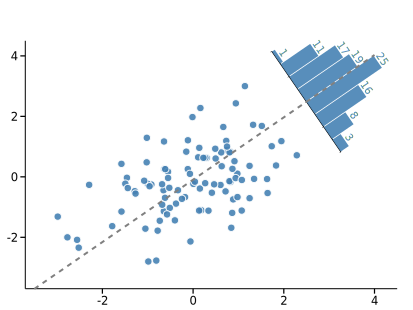
\includegraphics[width=0.55\textwidth]{./figs/pca.pdf}
\end{frame}

\begin{frame}{Introduction - Objective and Hypotheses}
    \textbf{Main Objective:} Develop a data visualization framework that extends the expressiveness of visualization grammars while preserving a high level of abstraction.
    \\[1em]
    \textbf{Hypothesis 1 (Cause):} Limitations in expressiveness are due to a lack of integration between graphic specification and assembly.
    \\[1em]
    \textbf{Hypothesis 2 (Solution):} Integration of diagramming and graphic specification via a unified constructive framework.
    \\[1em]
    \textbf{Formalization Tool:} Category Theory.
\end{frame}

\begin{frame}{Introduction - Overview}
    \centering
    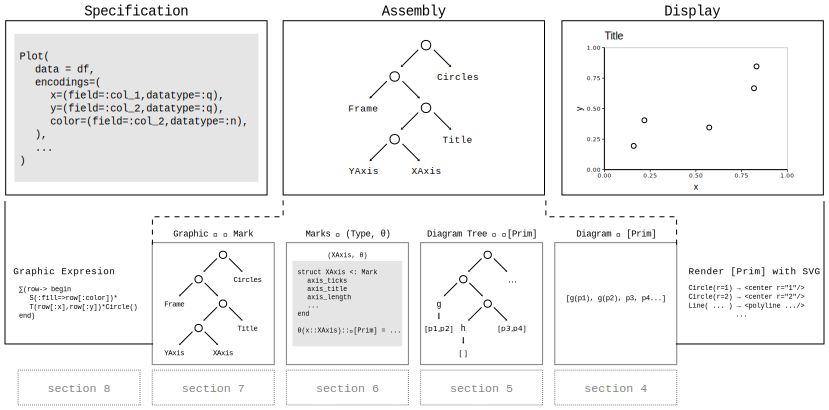
\includegraphics[width=0.9\textwidth]{figs/pipe.pdf}
\end{frame}

\begin{frame}{Data Visualization + Category Theory: Diagrams as Monoids}
    The basic building block for any diagram is the primitive.
    A primitive is any geometry that can be drawn and manipulated via geometric or stylistic transformations.
    \\[1em]
    \begin{center}
    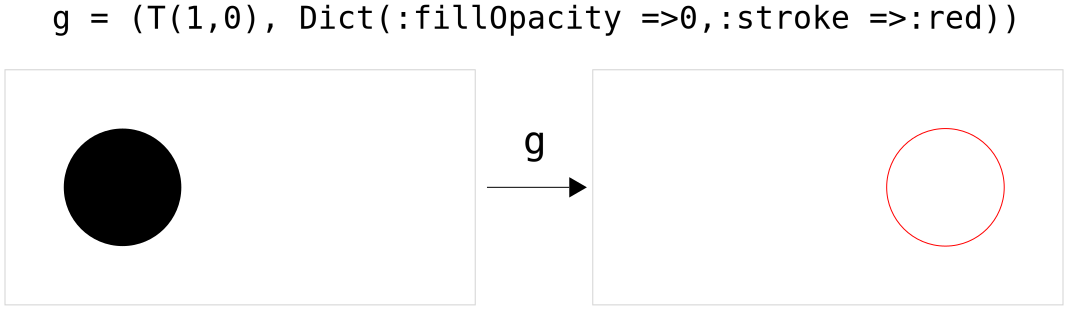
\includegraphics[width=0.7\textwidth]{figs/primitivetransformation.pdf}
    \end{center}
\end{frame}

\begin{frame}[fragile]{Data Visualization + Category Theory: Diagrams as Monoids}
    A diagram can be defined as an ordered list of primitives.
    $( [\text{Prim}] , +, [\ ] )$ can be interpreted as a monoid.
\begin{lstlisting}[language=JuliaLocal, style=julia, texcl=true, escapeinside={(@}{@)}]
abstract type Prim end
struct Circle <: Prim
  radius::Real
  center::Tuple{Real, Real}
end
+(d1::Vector{Prim}, d2::Vector{Prim}) = vcat(d1,d2)
\end{lstlisting}
\end{frame}

\begin{frame}[fragile]{Data Visualization + Category Theory: Diagrams as Monoids}

    Diagrams are drawn by rendering the list of primitives on top of each other.
    \begin{center}
        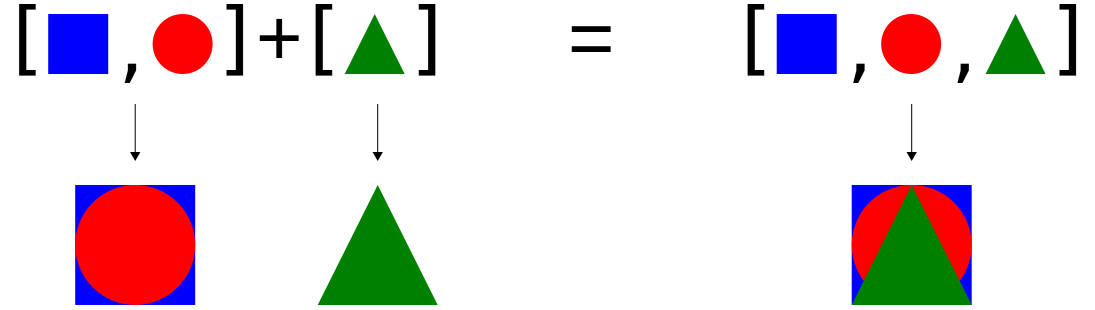
\includegraphics[width=0.7\textwidth]{./figs/simplediagram.pdf}
    \end{center}
\end{frame}

\begin{frame}[fragile]{Data Visualization + Category Theory: Diagrams as Monoids}

  We can apply transformations to diagrams by applying the
  transformations to each primitive in the list.
    \begin{center}
        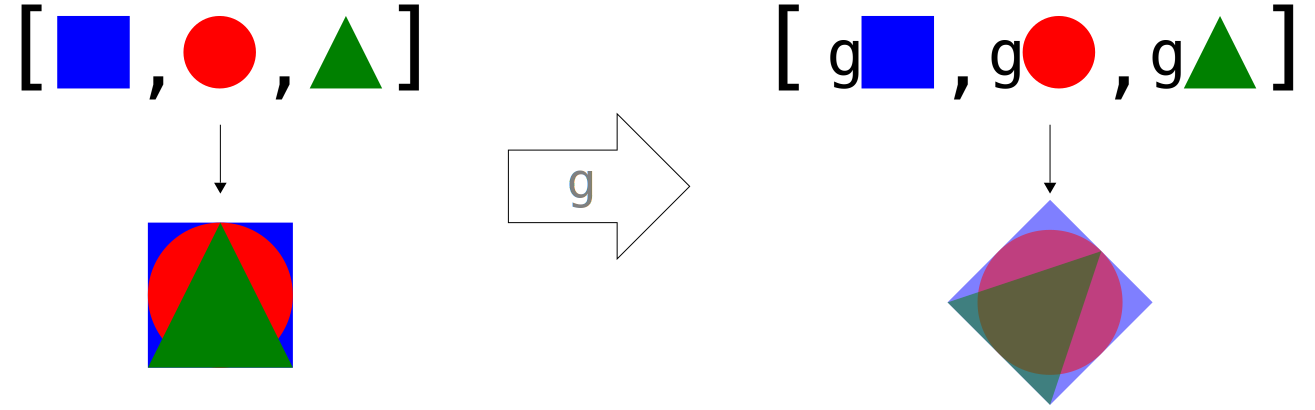
\includegraphics[width=0.7\textwidth]{./figs/diagramtransformation.pdf}
    \end{center}
\end{frame}

\begin{frame}[fragile]{Data Visualization + Category Theory}
    \centering
    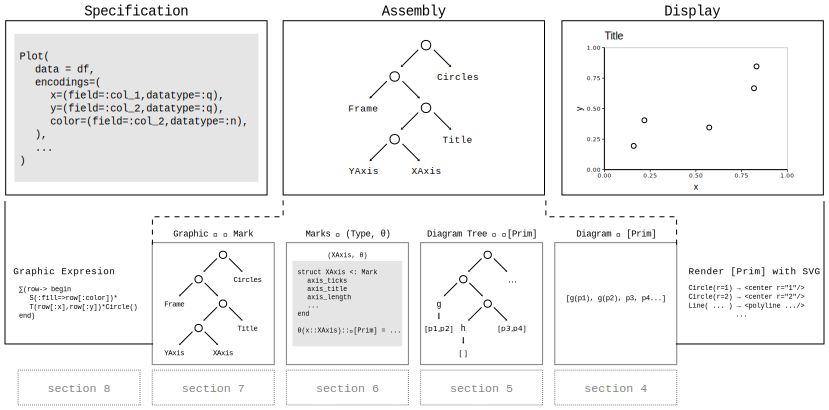
\includegraphics[width=0.9\textwidth]{figs/pipe.pdf}
\end{frame}

\begin{frame}[fragile]{Data Visualization + Category Theory: Free Monads}

  Let us improve our representation using expression trees.
  To do this, first we define a functor $F$ that encodes
  diagram composition (i.e. $+$) and diagram transformations.
\begin{lstlisting}[language=JuliaLocal, style=julia, texcl=true, escapeinside={(@}{@)}]
@data F{a} begin
Comp(::a, ::a)
Act(::H, ::a)
end
fmap(f::Function, x::Comp) = Comp(f(x._1),f(x._2))
fmap(f::Function, x::Act) = Act(x._1,f(x._2))
\end{lstlisting}

\end{frame}

\begin{frame}[fragile]{Data Visualization + Category Theory: Free Monads}

  Using our functor $F$, we can define a free monad over
  such functor, i.e $\mathbb T := \text{Free} F$. Thus,
  $(\mathbb T, \eta, \mu)$ is our monad, where $\mathbb T$ is a parametric type
  representing trees with $F$ as possible operations.

  To ease the process of expressing trees, we overload
  the $+$ and the $*$ operators to represent composition
  and transformation application respectively.

  \begin{figure}
    \begin{center}
        
\includegraphics[width=0.6\textwidth]{./figs/composetrees.pdf}
    \end{center}
  \end{figure}
  
\end{frame}

\begin{frame}[fragile]{Data Visualization + Category Theory: Free Monads}

    A diagram tree is a value of type $\mathbb T$ [Prim]. For this representation to
  be useful, we must be able to flatten it, i.e.
  we must define a function $f: \mathbb T\text{[Prim]} \to \text{[Prim]}$.
  We can do this using $F$-algebras and catamorphism.

  \begin{figure}
    \begin{center}
    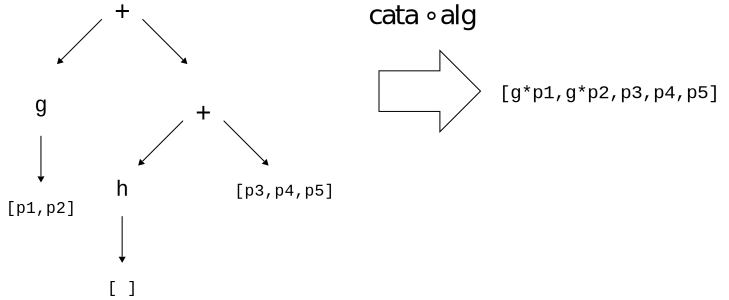
\includegraphics[width=0.7\textwidth]{./figs/flattree.pdf}
    \end{center}
  \end{figure}
\end{frame}

\begin{frame}[fragile]{Data Visualization + Category Theory}
    \begin{center}
    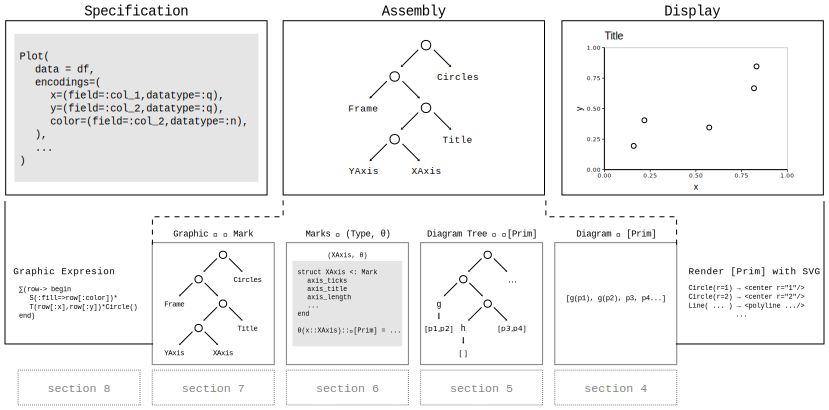
\includegraphics[width=0.9\textwidth]{./figs/pipe.pdf}
    \end{center}
\end{frame}


%------------------------------------------------
\begin{frame}{References}
    \footnotesize
    \bibliography{reference.bib}
    \bibliographystyle{apalike}
\end{frame}

%------------------------------------------------

% \begin{frame}
%     \Huge{\centerline{\textbf{The End}}}
% \end{frame}

%----------------------------------------------------------------------------------------

\end{document}
